\chapter{Macchine di Turing}

\subsubsection{Descrizione informale di una MdT}

Una macchina di Turing utilizza un nastro semi-infinito. Inizialmente il nastro contiene solo la stringa di input.
La macchina di Turing ha una testina di lettura e scrittura,
che può muoversi lungo il nastro.
In funzione dello stato in cui si trova e del simbolo input letto,
la macchina cambia stato, scrive un simbolo nella cella su cui
era posizionata, sposta la testina di una posizione a destra o a
sinistra.
La macchina continua a computare finché non accetta o
rifiuta.
Se non raggiunge uno stato corrispondente a uno delle due
situazioni precedenti, la computazione andrà avanti per
sempre.

\subsubsection{Schema di una Macchina di Turing}

\begin{figure}[hbpt!]
    \centering
    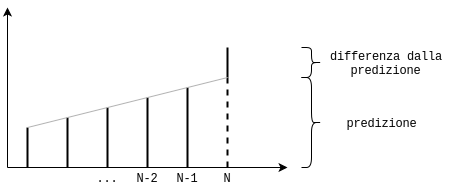
\includegraphics[width=9cm]{./Images/7.1.png}
\end{figure}
\FloatBarrier

\subsubsection{Differenze tra una MdT e un automa a stati finiti}
La definizione di Macchina di Turing (in seguito abbreviata con MdT o con TM) che daremo, metterà in evidenza le seguenti differenze con il modello automa finito:
\begin{itemize}
    \item  Una MdT ha un nastro semi-infinito (infinito a destra), diviso in celle, ciascuna contenente un carattere.
    \item Una MdT ha una testina che può muoversi a sinistra o a destra (ma non può oltrepassare il limite a sinistra del nastro).
    \item La testina può leggere o scrivere caratteri (testina di lettura-scrittura).
    \item Una MdT ha due stati speciali $q_{\text {accept }}, q_{\text {reject }}$ rispettivamente corrispondenti all'accettazione e al rifiuto della stringa input. Se la MdT si trova in uno di tali stati non può effettuare ulteriori passi di computazione. (La frase sul testo di Sipser è: Gli stati speciali di accettazione e rifiuto hanno effetto immediato.)
    \item Non c'è limite ai passi di computazione (in particolare il numero di tali passi non è limitato dalla lunghezza dell'input).
\end{itemize}

\subsubsection{Definizione di una MdT}

Una Macchina di Turing deterministica è una settupla
$\left(Q, \Sigma, \Gamma, \delta, q_{0}, q_{\text {accept }}, q_{\text {reject }}\right)$
dove:
\begin{itemize}
    \item Q: Insieme finito degli stati
    \item $\Sigma$ : Alfabeto dei simboli input $(\sqcup \notin \Sigma)$
    \item $\Gamma:$ Alfabeto (finito) dei simboli di nastro $(\sqcup \in \Gamma, \Sigma \subset \Gamma$, $L, R \notin \Gamma)$
    \item $\delta:\left(Q \backslash\left\{q_{\text {accept }}, q_{\text {reject }}\right\}\right) \times \Gamma \rightarrow Q \times \Gamma \times\{L, R\}:$ funzione transizione
    \item  $q_{0} \in Q$ : stato iniziale
\item $q_{\text {accept }} \in Q$ : stato di accettazione
\item $q_{\text {reject }} \in Q:$ stato di rifiuto, $q_{\text {accept }} \neq q_{\text {reject }}$
\end{itemize}

\subsubsection{Funzione di transizione di una MdT}

Sia $M=\left(Q, \Sigma, \Gamma, \delta, q_{0}, q_{\text {accept }}, q_{\text {reject }}\right)$ una MdT deterministica.

II suo comportamento è descritto dalla funzione di transizione
$\delta:\left(Q \backslash\left\{q_{\text {accept }}, q_{\text {reject }}\right\}\right) \times \Gamma \rightarrow Q \times \Gamma \times\{L, R\} .$
Se $\delta(q, \gamma)=\left(q^{\prime}, \gamma^{\prime}, d\right)$, sappiamo che $q, q^{\prime} \in Q, \gamma, \gamma^{\prime} \in \Gamma$, $d \in\{L, R\} .$

\vspace{5mm}

Se $\delta(q, \gamma)=\left(q^{\prime}, \gamma^{\prime}, d\right)$ e se $M$ si trova nello stato $q$ con la testina posizionata su una cella contenente $\gamma$, alla fine della transizione:
\begin{itemize}
    \item $M$ si troverà nello stato $q^{\prime}$,
    \item $\gamma^{\prime} \in \Gamma$ sarà il simbolo scritto sulla cella del nastro su cui la testina si trovava ALL'INIZIO della transizione (contenente $\gamma$ ),
    \item la testina si sarà spostata sulla cella di sinistra se (tale cella esiste e se) $d=L$, sulla cella di destra se $d=R$.
\end{itemize}
\textbf{NOTA:} Se $\delta(q, \gamma)=\left(q^{\prime}, \gamma^{\prime}, L\right)$, se $M$ si trova nello stato $q$ con la testina posizionata su una cella contenente $\gamma$ e se tale cella è quella più a sinistra del nastro, la testina non si sposta, resta sulla cella del nastro su cui si trovava all'inizio della transizione.

\subsubsection{Diagramma di stato di una MdT}

Come nel caso degli automi, spesso preferiamo utilizzare il diagramma di stato di una specifica Macchina di Turing piuttosto che la descrizione formale della settupla.

Il diagramma di stato di una Macchina di Turing è un grafo i cui nodi hanno come nomi gli stati della macchina.

Le etichette degli archi hanno la forma

"simbolo $\rightarrow$ simbolo, $d$ "


dove "simbolo" è un simbolo di $\Gamma$ e $d \in\{L, R\}$. Il simbolo a sinistra della freccia rappresenta il simbolo letto, quello dopo la freccia il simbolo (eventualmente lo stesso) che sostituisce il simbolo letto per effetto della transizione, $d$ lo spostamento per effetto della transizione.

\vspace{5mm}

Ad esempio se sull'arco dal nodo $q_{1}$ al nodo $q_{2}$ compare l'etichetta
$$
0 \rightarrow \sqcup, R
$$
questo corrisponde a
$$
\delta\left(q_{1}, 0\right)=\left(q_{2}, \sqcup, R\right)
$$
Alle volte si usa l'abbreviazione di non indicare il carattere dopo la freccia se esso non è modificato dalla transizione. Ad esempio se sull'arco dal nodo $q_{3}$ al nodo $q_{4}$ troviamo l'etichetta
$$
0 \rightarrow R
$$
questo vuol dire che
$$
\delta\left(q_{3}, 0\right)=\left(q_{4}, 0, R\right)
$$

\subsubsection{Esempio di Macchina di Turing}

\begin{figure}[hbpt!]
    \centering
    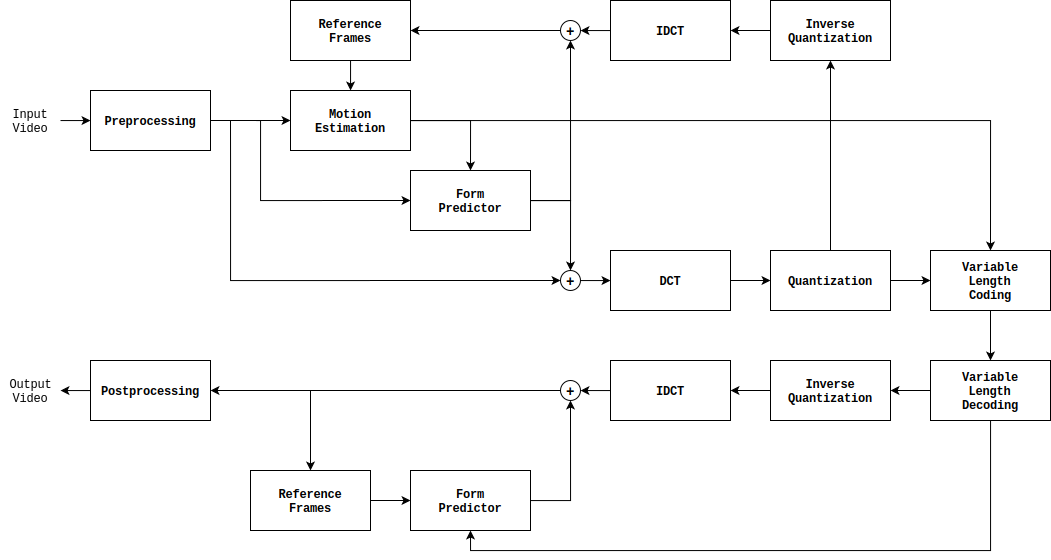
\includegraphics[width=9cm]{./Images/7.2.png}
\end{figure}
\FloatBarrier

\subsubsection{Computazione di una MdT - descrizione informale}

Una MdT M inizia la computazione:
\begin{itemize}
    \item partendo dallo stato iniziale $q_{0}$,
    \item con l'input $w \in \sum^{*}$ posizionato sulla parte più a sinistra del nastro: le prime $n$ celle a sinistra, se $n=|w|$ è la lunghezza dell'input (il resto delle celle conterrà il carattere $\sqcup$ ),
    \item con la testina posizionata sulla cella contenente il primo simbolo di input (quello più a sinistra).
\end{itemize}
La computazione termina se $M$ raggiunge
\begin{itemize}
    \item lo stato di accettazione $q_{\text {accept }}$ : Accetta input
    \item lo stato di rifiuto $q_{\text {reject }}$ : Rifiuta input
\end{itemize}

\textbf{NOTA:} La computazione può non terminare.

\subsubsection{Computazione di un automa finito deterministico}

La computazione di un automa finito deterministico su un input $w$ può essere rappresentata da una sequenza di stati (gli stati che rappresentano i nodi del cammino di etichetta $w$ nel diagramma di stato che rappresenta |'automa).

La posizione della testina è implicitamente rappresentata nella computazione poiché a ogni transizione si sposta di una cella a destra.

Il nastro è di sola lettura, il contenuto del nastro non viene modificato durante la computazione e quindi non è necessario considerarlo.

\subsubsection{Computazione di una MdT}

Nella computazione di una macchina di Turing su un input $w$ invece abbiamo bisogno di considerare tutti questi elementi:
\begin{itemize}
    \item stato
    \item posizione della testina
    \item la parte iniziale del nastro contenente tutti i caratteri diversi da $\sqcup($ eventualmente separati da $\sqcup)$.
    
Nota: è sempre costituita da un numero finito di celle.
\end{itemize}

Un'impostazione di questi tre elementi è chiamata una configurazione della macchina di Turing.

\subsubsection{Configurazione di una MdT}

Una configurazione $C$ di una $M d T$
$M=\left(Q, \Sigma, \Gamma, \delta, q_{0}, q_{\text {accept }}, q_{\text {reject }}\right)$ è una stringa
$C=u q v \in \Gamma^{*} Q \Gamma^{*}$, dove:
\begin{itemize}
    \item $q \in Q$ è lo stato corrente di $M$,
    \item $u v \in \Gamma^{*}$ è il contenuto del nastro
(con la convenzione di aver eliminato tutti i simboli $\sqcup$ dopo $v$, cioè dopo l'ultimo carattere di $v$ il nastro contiene solo simboli blank),
    \item la testina è posizionata sul primo simbolo di v.
\end{itemize}

\subsubsection{Computazione di una MdT}

\textbf{Passo di computazione}

Intuitivamente un passo di computazione è la trasformazione della configurazione $C_{1}$ nella configurazione $C_{2}$ per effetto di una applicazione della funzione di transizione.
E una relazione tra coppie di configurazioni definita dalla funzione di transizione.

\vspace{5mm}

Sia $M=\left(Q, \Sigma, \Gamma, \delta, q_{0}, q_{\text {accept }}, q_{\text {reject }}\right)$ una MdT deterministica.

Siano $q_{i}, q_{j} \in Q, a, b, c \in \Gamma$ e $u, v \in \Gamma^{*}$.

Diremo che $u a q_{i} b v$ produce $u q_{j} a c v$
se $\delta\left(q_{i}, b\right)=\left(q_{j}, c, L\right)$

Diremo che $u a q_{i} b v$ produce uacq $_{j} v$
se $\delta\left(q_{i}, b\right)=\left(q_{j}, c, R\right)$

Nota: $uaq_ibv, uq_j a c v, u a c q_{j} v$ sono configurazioni di $M$.

\vspace{5mm}

La definizione generale è più complessa perché bisogna considerare anche i casi particolari $(C=q v, C=u q$ con $u, v$ eventualmente uguali a $\epsilon$ ).

Ad esempio $q_{i} b v$ produce $q_{j} C v$ se $\delta\left(q_{i}, b\right)=\left(q_{j}, c, L\right)$.
$q_{i} b v$ produce $c q_{j} v$ se $\delta\left(q_{i}, b\right)=\left(q_{j}, c, R\right)$

Altri casi particolari: le configurazioni prodotte da $u q_{i}$. Occorre distinguere $u=\epsilon \mathrm{da} u \neq \epsilon$.

\vspace{5mm}

Siano $C_{1}, C_{2}$ due configurazioni di una MdT $M$.
Se $C_{1}$ produce $C_{2}$, scriveremo
$$
C_{1} \rightarrow C_{2}
$$
La trasformazione $\rightarrow$ di $C_{1}$ in $C_{2}$ prende il nome di passo di computazione.

Corrisponde a un'applicazione della funzione di transizione di $M .$

\vspace{5mm}

\textbf{Definizione}

Una configurazione $C$ si dice:
\begin{itemize}
    \item \textbf{iniziale} (con input w) se $C=q_{0} w$, con $w \in \Sigma^{*}$,
    \item \textbf{di arresto} se $C=u q v$, con $u, v \in \Gamma^{*} e q \in\left\{q_{\text {accept }}, q_{\text {reject }}\right\}$ (non esiste nessuna configurazione $C^{\prime}$ tale che $C \rightarrow C^{\prime}$ ),
    \item \textbf{di accettazione} se $C=u q v$, con $u, v \in \Gamma^{*}$ e $q=q_{\text {accept }}$,
    \item \textbf{di rifiuto} se $C=u q v$, con $u, v \in \Gamma^{*}$ e $q=q_{\text {reject }}$.
\end{itemize}

\textbf{Nota:} Le configurazioni di arresto sono configurazioni di accettazione o di rifiuto.

\vspace{5mm}

\textbf{Definizione}

Siano $C, C^{\prime}$ configurazioni.

$C \rightarrow^{*} C^{\prime}$ se esistono configurazioni $C_{1}, \ldots, C_{k}$ tali che
\begin{enumerate}
    \item $C_{1}=C$,
    \item $C_{i} \rightarrow C_{i+1}$, per $i \in\{1, \ldots, k-1\}$,
(ogni $C_{i}$ produce $C_{i+1}$ )
    \item $C_{k}=C^{\prime}$.
\end{enumerate}

Diremo che $C \rightarrow^{*} C^{\prime}$ è una computazione (di lunghezza $k-1) .$

\vspace{5mm}

Sia $M$ una MdT e sia C una configurazione di $M$. Ci sono tre possibili casi:
\begin{enumerate}
    \item $C \rightarrow^{*} C^{\prime} \operatorname{con} C^{\prime}=u q_{\text {accept }} v$ configurazione di accettazione (M si ferma in $\left.q_{\text {accept }}\right)$.
    \item$C \rightarrow^{*} C^{\prime} \operatorname{con} C^{\prime}=u q_{\text {reject }} v$ configurazione di rifiuto (M si ferma in $q_{\text {reject }}$ ).
    \item Per ogni configurazione $C^{\prime}$ tale che $C \rightarrow^{*} C^{\prime}$ esiste una configurazione $C^{\prime \prime}$ tale che $C \rightarrow^{*} C^{\prime} \rightarrow C^{\prime \prime}$ (M non si arresta).
\end{enumerate}

\subsubsection{Parola accettata da una MdT}

Una MdT M accetta una parola $w \in \Sigma^{*}$ se esiste una computazione $C \rightarrow^{*} C^{\prime}$, dove $C=q_{0} w$ è la configurazione iniziale di $M$ con input $w$ e $C^{\prime}=u q_{\text {accept }} v$ è una configurazione di accettazione.

\vspace{5mm}

Una MdT M rifiuta una parola $w \in \sum^{*}$ se esiste una computazione $C \rightarrow^{*} C^{\prime}$, dove $C=q_{0} w$ è la configurazione iniziale di $M$ con input $w$ e $C^{\prime}=u q_{\text {reject }} v$ è una configurazione di rifiuto.

\subsubsection{Linguaggio riconosciuto da una MdT}

Sia $M=\left(Q, \Sigma, \Gamma, \delta, q_{0}, q_{\text {accept }}, q_{\text {reject }}\right)$ una MdT. I/ linguaggio $L(M)$ riconosciuto da $M$, è l'insieme delle stringhe che $M$ accetta:

$L(M)=\left\{w \in \Sigma^{*} \mid \exists u, v \in \Gamma^{*} q_{0} w \rightarrow^{*} u q_{\text {accept }} v\right\}$


Quindi

$L(M)=\left\{w \in \Sigma^{*} \mid M\right.$ accetta $\left.w\right\} .$

\subsubsection{Linguaggi Turing riconoscibili e linguaggi decidibili}

Sia $R(M)=\left\{w \in \Sigma^{*} \mid M\right.$ rifiuta $\left.w\right\} .$
In generale $L(M) \cup R(M)$ non coincide con $\Sigma^{*}$.

Se $L(M) \cup R(M)=\Sigma^{*}$, allora $M$ si arresta su ogni input.

In tal caso $M$ è chiamata un decisore (o decider) ed $L(M)$ è il linguaggio deciso da $M$.

\vspace{5mm}

Occorre quindi definire due famiglie di linguaggi:

\vspace{5mm}

\textbf{Definizione}

Un linguaggio $L \subseteq \Sigma^{*}$ è Turing riconoscibile se esiste una macchina di Turing $M=\left(\bar{Q}, \Sigma, \Gamma, \delta, q_{0}, q_{\text {accept }}, q_{\text {reject }}\right)$ tale che:
\begin{enumerate}
    \item $M$ riconosce $L$ (cioè $\left.L=L(M)=\left\{w \in \Sigma^{*} \mid \exists u, v \in \Gamma^{*} q_{0} w \rightarrow^{*} u q_{\text {accept }} v\right\}\right)$.
\end{enumerate}


\vspace{5mm}

\textbf{Definizione}

Un linguaggio $L \subseteq \Sigma^{*}$ è decidibile se esiste una macchina di Turing $M=\left(Q, \Sigma, \Gamma, \delta, \bar{q}_{0}, q_{\text {accept }}, q_{\text {reject }}\right)$ tale che:
\begin{enumerate}
    \item $M$ riconosce $L$
(cioè $\left.L=L(M)=\left\{w \in \Sigma^{*} \mid \exists u, v \in \Gamma^{*} q_{0} w \rightarrow^{*} u q_{\text {accept }} v\right\}\right)$.
    \item $M$ si arresta su ogni input (cioè per ogni $w \in \Sigma^{*}, q_{0} w \rightarrow^{*}$ uqv con $\left.q \in\left\{q_{\text {accept }}, q_{\text {reject }}\right\}\right)$.
\end{enumerate}

L'insieme dei linguaggi decidibili è un sottoinsieme proprio dell'insieme dei linguaggi Turing riconoscibili.
Come conseguenza delle definizioni, un linguaggio L è Turing riconoscibile ma non decidibile se:
\begin{enumerate}
    \item esiste una MdT che riconosce $L$ (quindi accetta tutte e sole le stringhe $\operatorname{di} L$ )
    \item non esiste nessuna MdT $M$ tale che $M$ accetta tutte le stringhe in $L$ e rifiuta tutte le stringhe che appartengono al complemento $\bar{L}$ di $L$.
\end{enumerate}

\subsubsection{Macchine di Turing e Decider}

Una MdT $M=\left(Q, \Sigma, \Gamma, \delta, q_{0}, q_{\text {accept }}, q_{\text {reject }}\right)$ decide un linguaggio $L$ se per ogni $w \in \Sigma^{*}, q_{0} w \rightarrow^{*} C$ con $C=u q v$ configurazione di arresto ed $L=L(M)$.

In questo caso diciamo che $L$ è il linguaggio deciso da $M$.

\vspace{5mm}

\textbf{Nota:} data una MdT $M$, esiste sempre il linguaggio riconosciuto da $M$ ma non è detto che esista il linguaggio deciso da $M$, ciò è possibile se e solo se $M$ è un decider.

Se $M$ è un decider, esiste il linguaggio deciso da $M$ e coincide con il linguaggio riconosciuto da $M$.

Se $M$ non è un decider, esiste il linguaggio riconosciuto da $M$ ma non il linguaggio deciso da $M$.

\subsubsection{Funzioni calcolabili}

Una funzione $f: \Sigma^{*} \rightarrow \Sigma^{*}$ è calcolabile se esiste una macchina di Turing $M=\left(Q, \Sigma, \Gamma, \delta, q_{0}, q_{\text {accept }}, q_{\text {reject }}\right)$ tale che
$\forall w \in \Sigma^{*} \quad q_{0} w \rightarrow^{*} q_{\text {accept }} f(w)$

\vspace{5mm}

Quindi, una funzione $f: \Sigma^{*} \rightarrow \Sigma^{*}$ è calcolabile se esiste una macchina di Turing $M$ che, su qualsiasi input $w$, si ferma avendo solo $f(w)$ sul nastro.

\textbf{Nota:} in questo caso la MdT deve arrestarsi su ogni input.
\begin{itemize}
    \item Possibile variante: nessun vincolo sulla posizione della testina nella configurazione di arresto.
    \item Possibile variante: nessuna distinzione tra qaccept e $q_{\text {reject }}$.
\end{itemize}

\section{Varianti di Macchine di Turing}

Esistono diverse varianti della definizione di macchina di
Turing deterministica.
Ad esempio:
\begin{itemize}
    \item la Macchina di Turing multinastro
    \item la Macchina di Turing non deterministica
\end{itemize}

Tali macchine di Turing hanno lo stesso potere
computazionale (o espressivo) delle MdT deterministiche, cioè
riconoscono la stessa classe di linguaggi.
Esistono anche altre varianti della macchina di Turing
deterministica che hanno lo stesso potere espressivo.

Questa "robustezza" rispetto ai cambiamenti è una conferma
che si tratta di un buon modello per la definizione di
algoritmo.

\subsubsection{Un semplice esempio}

Consideriamo una variante della definizione data di macchina di Turing deterministica. Sia $\mathcal{T}_{(L, R)}$ |'insieme delle macchine di Turing che abbiamo definito e sia $\mathcal{T}_{(L, R, S)}$ l'insieme i cui elementi $M$ sono definiti al modo seguente:

$M=\left(Q, \Sigma, \Gamma, \delta, q_{0}, q_{\text {accept }}, q_{\text {reject }}\right)$ è una settupla dove $Q, \Sigma, \Gamma, q_{0}, q_{a c c e p t}, q_{r e j e c t}$ sono definiti come in una MdT deterministica e la funzione di transizione $\delta$ è definita al modo seguente:

$\delta:\left(Q \backslash\left\{q_{\text {accept }}, q_{\text {reject }}\right\}\right) \times \Gamma \rightarrow Q \times \Gamma \times\{L, R, S\}$

\vspace{5mm}

Se $\delta(q, \gamma)=\left(q^{\prime}, \gamma^{\prime}, d\right)$ e se $M$ si trova nello stato $q$ con la testina posizionata su una cella contenente $\gamma$, alla fine della transizione:
\begin{itemize}
    \item $M$ si troverà nello stato $q^{\prime}$,
    \item $\gamma^{\prime} \in \Gamma$ sarà il simbolo scritto sulla cella del nastro su cui la testina si trovava all'inizio della transizione (contenente $\gamma$ ),
    \item la testina si troverà sulla stessa cella cui si trovava all'inizio della computazione se $d=S$, si sarà spostata sulla cella di sinistra se (tale cella esiste e se) $d=L$, si sarà spostata sulla cella di destra se $d=R$.
\end{itemize}

Le nozioni di configurazione, di linguaggio deciso e di linguaggio riconosciuto da $M^{\prime} \in \mathcal{T}_{(L, R)}$ sono estese in maniera ovvia alle macchine $M$ in $\mathcal{T}_{(L, R, S)}$.

\vspace{5mm}

I modelli in $\mathcal{T}_{(L, R)}$ hanno lo stesso potere computazionale dei modelli in $\mathcal{T}_{(L, R, S)}$.
Se $M^{\prime} \in \mathcal{T}_{(L, R)}$, esiste $M \in \mathcal{T}_{(L, R, S)}$ tale che $L(M)=L\left(M^{\prime}\right)$.

Viceversa se $M \in \mathcal{T}_{(L, R, S)}$ esiste $M^{\prime} \in \mathcal{T}_{(L, R)}$ tale che $L\left(M^{\prime}\right)=L(M) .$

\subsection{Macchina di Turing multinastro}

Una macchina di Turing multinastro (abbreviata MdTM) è una
macchina di Turing in cui si hanno più nastri contemporaneamente
accessibili in scrittura e lettura che vengono aggiornati tramite più
testine (una per nastro).

\vspace{5mm}

Dato un numero naturale $k$, una macchina di Turing con $k$ nastri è una settupla
$$
\left(Q, \Sigma, \Gamma, \delta, q_{0}, q_{\text {accept }}, q_{\text {reject }}\right)
$$
dove $Q, \Sigma, \Gamma, q_{0}, q_{\text {accept }}, q_{\text {reject }}$ sono definiti come in una MdT deterministica e la funzione di transizione $\delta$ è definita al modo seguente:
$$
\delta:\left(Q \backslash\left\{q_{\text {accept }}, q_{\text {reject }}\right\}\right) \times \Gamma^{k} \rightarrow Q \times \Gamma^{k} \times\{L, R, S\}^{k}
$$
Nota: $\Gamma^{k}$ è il prodotto cartesiano di $k$ copie di $\Gamma$ e $\{L, R, S\}^{k}$ è il prodotto cartesiano di $k$ copie di $\{L, R, S\}$.

\vspace{5mm}

\textbf{Definizione (MdT multinastro)}

Una macchina di Turing multinastro è una macchina di Turing a $k$ nastri, con $k \in \mathbb{N}$.

%%%%%%%%%%immagine
\begin{figure}[hbpt!]
    \centering
    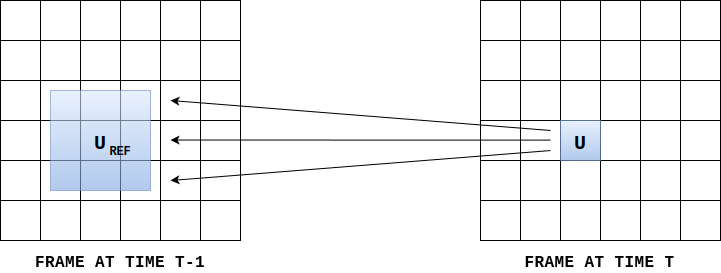
\includegraphics[width=9cm]{./Images/7.3.png}
\end{figure}
\FloatBarrier

\subsubsection{Funzione di transizione di una MdTM}

Il codominio della funzione di transizione è un insieme di sequenze $\left(q_{j}, b_{1}, \ldots, b_{k}, d_{1}, \ldots, d_{k}\right)$ di lunghezza $(2 k+1)$ dove:
\begin{itemize}
    \item $q_{j} \in Q$
    \item $b_{t} \in \Gamma$, per $t \in\{1, \ldots, k\}$
    \item $d_{t} \in\{L, R, S\}$, per $t \in\{1, \ldots, k\}$
\end{itemize}

Se $\delta\left(q_{i}, a_{1}, \ldots, a_{k}\right)=\left(q_{j}, b_{1}, \ldots, b_{k}, d_{1}, \ldots, d_{k}\right)$ e se $M$ si trova nello stato $q_{i}$ con le $k$ testine - una per nastro -
posizionate su celle contenente $a_{1}, \ldots, a_{k}$ rispettivamente, alla fine della transizione:
\begin{itemize}
    \item M si troverà nello stato $q_{j}$,
    \item $b_{t} \in \Gamma$ sarà il simbolo scritto sulla cella del $t$-esimo nastro su cui la testina si trovava all'inizio della transizione (contenente $\left.a_{t}\right)$, per $t \in\{1, \ldots, k\}$
    \item la testina sul $t$-esimo nastro si troverà sulla stessa cella cui si trovava all'inizio della computazione se $d_{t}=S$, si sarà spostata sulla cella di sinistra se (tale cella esiste e se) $d_{t}=L$, si sarà spostata sulla cella di destra se $d_{t}=R$, per $t \in\{1, \ldots, k\}$.
\end{itemize}


\subsubsection{Computazione di una MdTM}

Una MdTM inizia la computazione:
\begin{itemize}
    \item partendo dallo stato iniziale $q_{0}$,
    \item con l'input $w \in \Sigma^{*}$ posizionato sulla parte più a sinistra del primo nastro: le prime $n$ celle a sinistra, se $n=|w|$ è la lunghezza dell'input (il resto delle celle conterrà il carattere $\sqcup$ )
    \item Gli altri nastri conterranno solo il carattere $\sqcup$
    \item la testina del primo nastro sarà posizionata sulla cella contenente il primo simbolo di input (quello più a sinistra), le altre sulla prima cella dei rispettivi nastri.
\end{itemize}

Le nozioni di configurazione, passo di computazione, di linguaggio deciso e di linguaggio riconosciuto da una MdT sono estese in maniera ovvia alle macchine MdTM.
$$
\begin{aligned}
L(M)=&\left\{w \in \Sigma^{*} \mid \exists u_{t}, v_{t} \in \Gamma^{*}, t \in\{1, \ldots, k\}:\right.\\
&\left.\left(q_{0} w, \ldots, q_{0}\right) \rightarrow^{*}\left(u_{1} q_{\text {accept }} v_{1}, \ldots, u_{k} q_{\text {accept }} v_{k}\right)\right\} .
\end{aligned}
$$

\subsubsection{MdTM e MdT}

\textbf{Teorema}

Per ogni macchina di Turing multinastro $M$ esiste una macchina di Turing (a nastro singolo) $M^{\prime}$ equivalente ad $M$, cioè tale che $L(M)=L\left(M^{\prime}\right) .$

\begin{figure}[hbpt!]
    \centering
    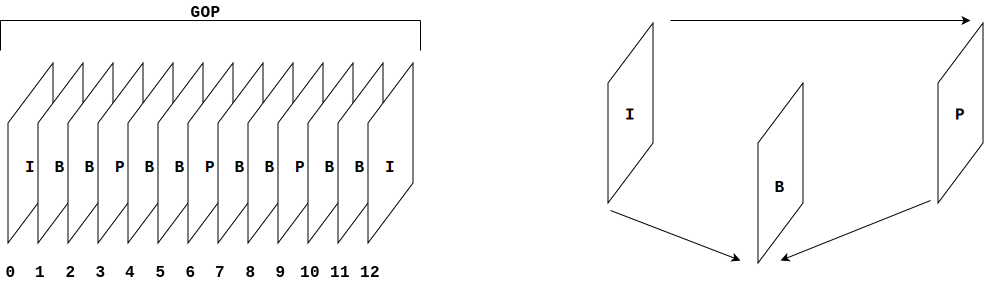
\includegraphics[width=9cm]{./Images/7.4.png}
\end{figure}
\FloatBarrier

\textbf{Teorema}

Un linguaggio L è Turing riconoscibile se e solo se esiste una macchina di Turing multinastro $M$ che lo riconosce, cioè tale che $L(M)=L .$

\subsection{Macchina di Turing non deterministica}

Introduciamo una variante della macchina di Turing deterministica, detta macchina di Turing non deterministica. Essenzialmente, una macchina di Turing non deterministica differisce da una deterministica per il fatto che una configurazione può evolvere in più di una configurazione successiva.

Le macchine non deterministiche hanno lo stesso potere computazionale di quelle deterministiche.
Tuttavia le macchine di Turing deterministiche possono simulare quelle non deterministiche con una perdita di efficienza esponenziale.

\vspace{5mm}

Una Macchina di Turing non deterministica è una settupla $\left(Q, \Sigma, \Gamma, \delta, q_{0}, q_{\text {accept }}, q_{\text {reject }}\right)$ dove:
\begin{itemize}
    \item Q, $\Sigma, \Gamma, q_{0}, q_{\text {accept }}, q_{\text {reject }}$ sono definiti come in una MdT deterministica
    \item la funzione di transizione $\delta$ è definita al modo seguente:
    $$
\delta:\left(Q \backslash\left\{q_{\text {accept }}, q_{\text {reject }}\right\}\right) \times \Gamma \rightarrow \mathcal{P}(Q \times \Gamma \times\{L, R\})
$$
\end{itemize}
Quindi per ogni $q \in Q \backslash\left\{q_{\text {accept }}, q_{\text {reject }}\right\}$, per ogni $\gamma \in \Gamma$, risulta $\delta(q, \gamma)=\left\{\left(q_{1}, \gamma_{1}, d_{1}\right), \ldots,\left(q_{k}, \gamma_{k}, d_{k}\right)\right\}$, con $k \geq 0$ e $\left(q_{j}, \gamma_{j}, d_{j}\right) \in Q \times \Gamma \times\{L, R\}$, per $j \in\{1, \ldots, k\} .$

\vspace{5mm}

Le configurazioni hanno la stessa forma uqv di quelle definite per una Macchina di Turing deterministica.
Allo stesso modo non cambia il passo di computazione $C_{1} \rightarrow C_{2}$ e una computazione $C \rightarrow^{*} C^{\prime}$ continua a essere una successione finita (non un albero!) di configurazioni.

Poiché però la macchina di Turing è non deterministica, ci possono essere più configurazioni $u^{\prime} q^{\prime} v^{\prime}$ che sono prodotte da uqv in un solo passo.

\vspace{5mm}

Quindi, come in un NFA, le computazioni (a partire da una configurazione) possono essere organizzate in un albero in cui la radice è la configurazione di partenza (tipicamente quella iniziale), i nodi sono configurazioni i cui figli rappresentano le possibili configurazioni raggiungibili da quel nodo.
Una computazione è completamente determinata da una sequenza di scelte tra le varie configurazioni raggiungibili passo dopo passo.
Quindi una computazione può essere rappresentata da un cammino nell'albero.

\subsubsection{Linguaggio riconosciuto da una MdT non deterministica}

\textbf{Definizione}

Sia $M=\left(Q, \Sigma, \Gamma, \delta, q_{0}, q_{\text {accept }}, q_{\text {reject }}\right)$ una MdT non deterministica. II linguaggio $L(M)$ riconosciuto da $M$, è l'insieme:


$L(M)=\left\{w \in \Sigma^{*} \mid \exists\right.$ una computazione $\left.q_{0} w \rightarrow^{*} C \operatorname{con} C=u q_{\text {accept }} v\right\}$

\begin{itemize}
    \item Come per le macchine di Turing deterministiche, partendo dalla configurazione $q_{0} w$, la computazione può terminare (se si raggiunge una configurazione di arresto) o non terminare. La stringa appartiene ad $L(M)$ se esiste una successione di scelte tali che $q_{0} w \rightarrow^{*} C$, con $C$ configurazione di accettazione.
    \item Non sono considerate funzioni calcolate da una MdT non deterministica.
\end{itemize}

\subsubsection{Linguaggio riconosciuto e linguaggio deciso da una MdT
non deterministica}

Anche per le macchine di Turing non deterministiche sono definite due famiglie di linguaggi:
\begin{itemize}
    \item I linguaggi $L$ riconosciuti da macchine di Turing non deterministiche, cioè tali che esiste una MdT non deterministica $M$ con $L=L(M)$
    \item I linguaggi $L$ decisi da macchine di Turing non deterministiche. Un linguaggio $L \subseteq \Sigma^{*}$ è deciso da una macchina di Turing non deterministica $M=\left(Q, \Sigma, \Gamma, \delta, q_{0}, q_{a c c e p t}, q_{r e j e c t}\right)$ se $M$ è tale che:
    \begin{enumerate}
        \item per ogni $w \in \Sigma^{*}$, per ogni $q_{0} w \rightarrow^{*} C^{\prime}$ esiste $C=u q v$ tale che $q \in\left\{q_{\text {accept }}, q_{\text {reject }}\right\}$ e $q_{0} w \rightarrow{ }^{*} C^{\prime} \rightarrow{ }^{*} C$ (tutte le computazioni a partire da $q_{0} w$ terminano in una configurazione di arresto)
        \item $M$ riconosce $L$ (cioè $L=L(M)=\left\{w \in \Sigma^{*} \mid \exists\right.$ una computazione $q_{0} w \rightarrow^{*}$ $C$ con $\left.\left.C=u q_{\text {accept }} v\right\}\right)$.
    \end{enumerate}
\end{itemize}

\subsubsection{Macchina di Turing non deterministica}

\textbf{Teorema}

Per ogni macchina di Turing non deterministica $N$ esiste una macchina di Turing deterministica $D$ equivalente ad $N$, cioè tale che $L(N)=L(D)$.

\begin{figure}[hbpt!]
    \centering
    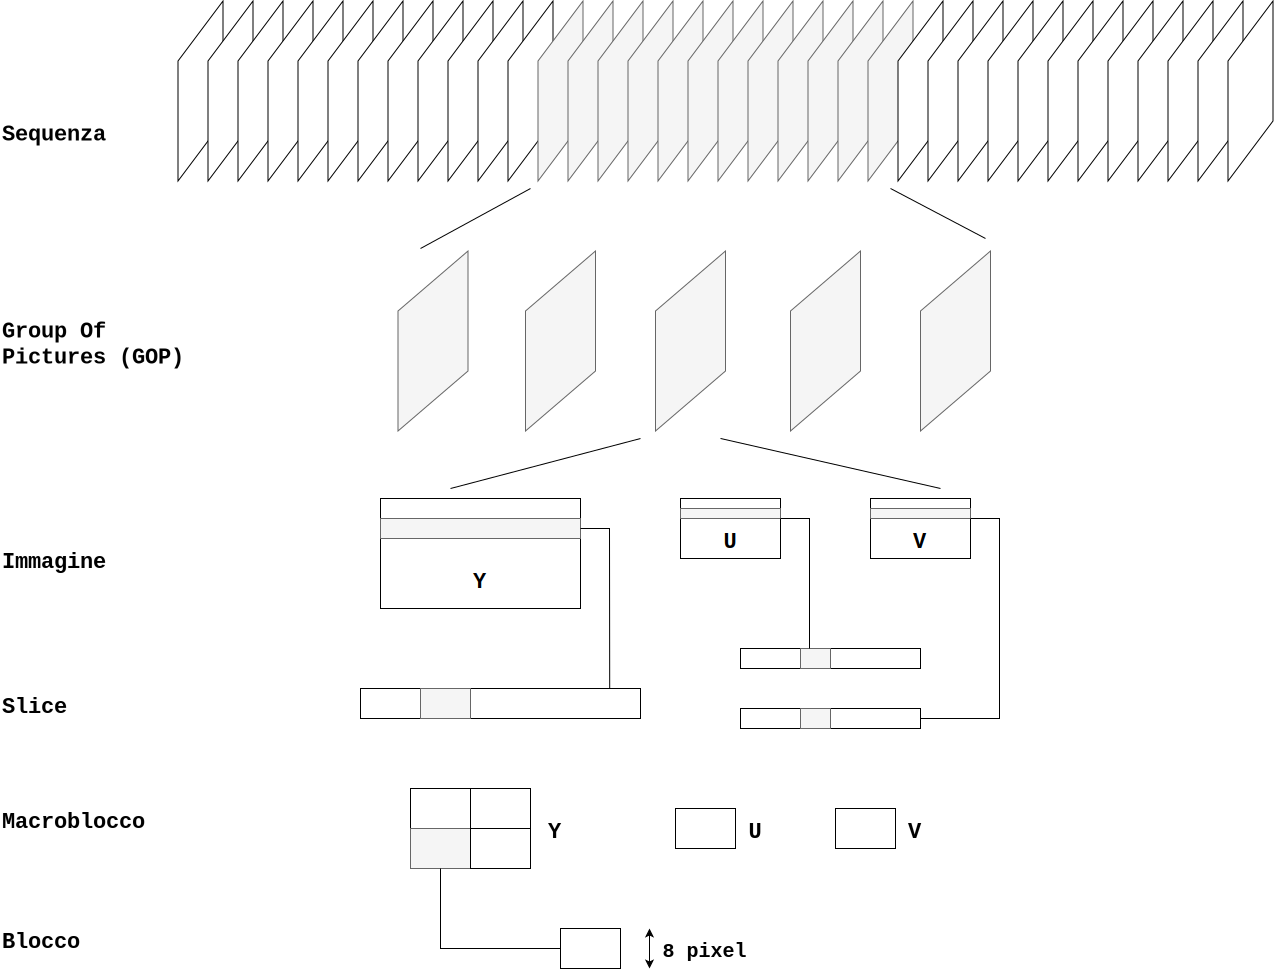
\includegraphics[width=9cm]{./Images/7.5.png}
\end{figure}
\FloatBarrier

\textbf{Corollario}

Un linguaggio $L$ è Turing riconoscibile se e solo se esiste una macchina di Turing non deterministica $N$ che lo riconosce, cioè tale che $L(N)=L$.

\vspace{5mm}

Una macchina di Turing non deterministica $N$ può essere simulata da una MdT deterministica $D$. E possibile modificare la prova di questo risultato per provare che se $N$ è una macchina di Turing non deterministica tale che, per ogni input $w, N$ si ferma sempre su tutte le ramificazioni dell'albero delle computazioni su $w$, allora esiste una MdT deterministica $D$ che simula $N$ e che si arresta su ogni input (cioè $D$ è un decisore). Diremo che una macchina di Turing non deterministica è un decisore se tutte le sue ramificazioni si fermano su ogni input.

\vspace{5mm}


\textbf{Corollario}

Un linguaggio $L$ è decidibile se e solo se esiste una macchina di Turing non deterministica $N$ che lo decide.


\subsection{Altre varianti equivalenti}

Altri esempi di varianti equivalenti sono:
\begin{itemize}
    \item Macchina di Turing con nastro infinito (in entrambe le direzioni).
    \item Macchina di Turing con $|\Sigma|=1$.
    \item Enumeratori (varianti di macchine di Turing per generare le stringhe in un linguaggio).
\end{itemize}

\subsubsection{La definizione di algoritmo}
\begin{itemize}
    \item Algoritmi per eseguire calcoli in svariati campi erano noti già nell'antichità (esempio: Algoritmo di Euclide per il calcolo del MCD, circa 300 A.C.).
Turing ha il merito di aver definito in modo formale il concetto di algoritmo.
    \item L'esigenza nacque a causa di un problema posto da Hilbert, al Congresso internazionale di Matematica del 1900 (Parigi), il decimo di una lista di 23 problemi:
(Decimo problema di Hilbert) progettare un algoritmo per decidere se un polinomio ha radici in $\mathbb{Z}$.
Esempio: $6 x^{3} y z^{2}+3 x y^{2}-x^{3}-10$ ammette la radice $x=5$, $y=3, z=0$.
    \item Vi era l'assunzione implicita che ogni enunciato potesse essere provato o confutato mediante un algoritmo.
\end{itemize}
\textbf{Nota: }per provare che un problema è risolubile mediante un algoritmo basta esibire l'algoritmo.
Per provare che per un problema non esiste nessun algoritmo che lo risolve, è necessario definire in modo formale la nozione di algoritmo.

\vspace{5mm}

Risolvendo negativamente un altro problema posto da Hilbert nel 1928 (il problema della decisione), Turing introdusse nel 1936 il modello formale che da lui prende il nome.
Usando tale modello e basandosi sul lavoro di Davis, Putnam e Robinson, molti anni dopo (1970), Matijasevic provò l'indecidibilità del decimo problema: non esiste nessun algoritmo per decidere se un polinomio ha radici intere.

\subsubsection{Equivalenza con altri modelli}

Molti altri modelli formali per la definizione di algoritmo
furono dati negli stessi anni 30:
\begin{itemize}
    \item i sistemi di Post (da Post)
    \item le funzioni $\mu$-ricorsive (Godel, Herbrand)
    \item il $\lambda$-calcolo (Church, Kleene)
    \item la logica combinatoria (Schonfinkel, Curry)
\end{itemize}

Fu dimostrato che tutti questi modelli erano equivalenti, cioè
conducevano alla stessa classe di problemi risolvibili mediante
algoritmi.

\subsubsection{Tesi di Church}

L'equivalenza dei vari modelli proposti condusse alla
Tesi di Church (o Tesi di Church-Turing): La macchina di Turing è la definizione formale della nozione intuitiva di algoritmo.

La tesi di Church non è un teorema ed è indimostrabile. Tenendo conto che essa è antecedente alla costruzione dei primi computer, costitui un enorme salto intellettuale.
L'evoluzione dei sistemi di calcolo ha generato negli ultimi anni una corrente di studi rivolti al superamento (o alla integrazione) del modello di Turing.

\section{Problemi e Linguaggi - Problemi di decisione}

Un problema di decisione è un problema che ha come soluzione una risposta sì o no.
Esempi:
\begin{itemize}
    \item Problema PRIMO: Dato un numero $x$ intero e maggiore di uno, $x$ è primo?
    \item  Problema CONNESSO: Dato un grafo $G, G$ è connesso?
    \item Problema A DFA: Dato un DFA $\mathcal{B}$ e una stringa $w, \mathcal{B}$ accetta w?
\end{itemize}

\subsubsection{Richiami di logica}

\begin{itemize}
    \item Variabili Booleane: variabili che possono assumere valore 1 (o TRUE ) o ( O FALSE)
    \item Operazioni Booleane: $\vee( O R), \wedge( A N D), \neg( N O T)$
    \item Denotiamo $\neg x \operatorname{con} \bar{x}$.
\end{itemize}

\textbf{Definizione}

Dato un insieme di variabili booleane $X$, le formule booleane espressioni booleane) su $X$ sono definite ricorsivamente come segue:
\begin{itemize}
    \item le costanti 0, 1 e le variabili (in forma diretta o complementata) $x, \bar{x}, \operatorname{con} x \in X$, sono formule booleane.
    \item Se $\phi, \phi_{1}, \phi_{2}$ sono formule booleane allora $\left(\phi_{1} \vee \phi_{2}\right),\left(\phi_{1} \wedge \phi_{2}\right)$, $\bar{\phi}$ sono formule booleane.
\end{itemize}

Una formula booleana $\phi$ è \textbf{soddisfacibile} se esiste un insieme di valori 0 o 1 per le variabili di $\phi$ (o assegnamento) che renda la formula uguale a 1 (assegnamento di soddisfacibilità). Diremo che tale assegnamento soddisfa $\phi$ o anche che rende vera $\phi$.
Esempi:
\begin{itemize}
    \item $\phi_{1}=(\bar{x} \vee y) \wedge(x \vee \bar{z})$ è soddisfacibile (assegnamento: $x=0$, $y=1, z=0)$,
    \item $\phi_{2}=(\bar{x} \wedge y) \vee(x \wedge \bar{z})$ è soddisfacibile,
    \item $\phi_{3}=(\bar{x} \vee x) \wedge(y \vee \bar{y})$ è soddisfacibile (per qualunque assegnamento di valori delle variabili),
    \item $\phi_{4}=\left(x_{1} \vee x_{2}\right) \wedge\left(x_{1} \vee \overline{x_{2}}\right) \wedge\left(\overline{x_{1}} \vee x_{2}\right) \wedge\left(\overline{x_{1}} \vee \overline{x_{2}}\right)$ non è soddisfacibile.
\end{itemize}

\subsubsection{Problemi di decisione}

Una formula booleana $\phi$ è soddisfacibile se esiste un assegnamento di valori di verità $F \circ T$ alle variabili di $\phi$ che soddisfa $\phi$, cioè che renda la formula uguale a $T$.

- Problema SAT: Data una formula booleana $\phi, \phi$ è soddisfacibile?

\vspace{5mm}

Un cammino Hamiltoniano in un grafo orientato è un cammino (orientato) che passa per ogni vertice del grafo una e una sola volta.

- Problema HAMPATH: Dato un grafo orientato $G$ e due vertici $s$ e $t$, esiste un cammino hamiltoniano nel grafo da $s$ a $t ?$

\vspace{5mm}

Un problema di decisione considera elementi di un insieme. Tali elementi sono anche chiamati le istanze del problema.
Quindi un istanza di un problema è un particolare input per quel problema.
\begin{itemize}
    \item Esempio: 3, 4, 6 sono istanze per il problema PRIMO.
    \item Esempio: $\left(x_{1} \vee x_{2}\right) \wedge\left(\overline{x_{1}} \vee x_{2}\right)$ è un istanza per il problema SAT.
\end{itemize}

L'insieme delle istanze (per un problema di decisione) è unione del sottoinsieme delle istanze con risposta sì e del sottoinsieme delle istanze con risposta no.
\begin{itemize}
    \item Esempio: 3 è un'istanza sì per il problema PRIMO, 4 e 6 sono istanze no per il problema PRIMO.
    \item Esempio: $\left(x_{1} \vee x_{2}\right) \wedge\left(x_{1} \vee x_{2}\right)$ è un istanza sì per il problema SAT (prendere $x_{1}=x_{2}=T$ ).
$$
\left(x_{1} \vee x_{2}\right) \wedge\left(x_{1} \vee \overline{x_{2}}\right) \wedge\left(\overline{x_{1}} \vee x_{2}\right) \wedge\left(\overline{x_{1}} \vee \overline{x_{2}}\right)
$$
è un istanza no per il problema SAT.
\end{itemize}

\subsubsection{Altri esempi}
\begin{itemize}
    \item Nel problema PRIMO le istanze sono i numeri $x$ interi e maggiori di uno.
L'insieme $\{n \in \mathbb{N} \mid n>1\}$ di tali numeri è unione dell'insieme dei numeri primi (istanze si) e dell'insieme dei numeri non primi o composti (istanze no).
    \item Nel problema CONNESSO le istanze sono grafi $G$. L'insieme dei grafi è unione dell'insieme dei grafi connessi (istanze sì) e dell'insieme dei grafi non connessi (istanze no).
    \item Nel problema A DFA le istanze sono coppie $(\mathcal{B}, w)$ costituite da un DFA $\mathcal{B}$ e da una stringa $w$.
L'insieme di tali coppie $(\mathcal{B}, w)$ è unione dell'insieme delle $(\mathcal{B}, w)$ con $w \in L(\mathcal{B})$ (istanze si) e dell'insieme delle $(\mathcal{B}, w)$ con $w \notin L(\mathcal{B})$ (istanze no).
\end{itemize}

\subsubsection{Problemi di decisione e ricerca di una soluzione}

In realtà in generale siamo interessati a trovare una soluzione
piuttosto che a sapere se c'è una soluzione.
Chiamiamo problemi di ricerca quelli per i quali cerchiamo una
soluzione (se esiste).

\begin{itemize}
    \item \textbf{Esempio} 
RSAT: Data una formula booleana $\phi$, fornire, se esiste, un assegnamento di valori di verità che soddisfa $\phi$.
    \item \textbf{Esempio}
RHAMPATH: Dato un grafo orientato $G$ e due vertici $s$ e $t$, fornire, se esiste, un cammino hamiltoniano nel grafo da $s$ a $t$.
\end{itemize}
Dato un problema di ricerca possiamo in genere usare come
sottoprogramma un algoritmo per il corrispondente problema di
decisione, se tale algoritmo esiste (altrimenti né l'uno né l'altro è
algoritmicamente risolubile).
Questo giustifica la concentrazione sui problemi di decisione.

\vspace{5mm}

Esempio: Data una formula booleana $\phi$, vogliamo fornire, se esiste, un assegnamento di valori di verità che soddisfa $\phi$. Disponiamo di un algoritmo Al che risolve SAT. Usiamo Al per stabilire se $\phi$ è soddisfacibile. Se $\phi$ non è soddisfacibile abbiamo una risposta al nostro problema di ricerca: l'assegnamento non esiste. Se $\phi$ è soddisfacibile
\begin{enumerate}
    \item Assegniamo a una delle variabili $x$ il valore $T$.
    \item Eseguiamo Al sulla nuova formula ottenuta.
    \item Se tale formula non è soddisfacibile, assegniamo a $x$ il valore $F$. La formula ottenuta sarà ora soddisfacibile perché se $\phi$ è soddisfacibile, uno dei due valori è quello giusto.
    \item Chiamiamo $\phi^{\prime}$ la formula ottenuta da $\phi$ assegnando in essa a $x$ il "giusto" valore. Se in $\phi^{\prime}$ vi sono ancora variabili, riapplichiamo la procedura dal passo 1 a $\phi^{\prime}$.
\end{enumerate}

\subsection{Linguaggio associato a un problema di
decisione}

La teoria della decidibilità si pone l'obiettivo di analizzare i
limiti della risoluzione dei problemi mediante algoritmi, cioè di
mostrare l'esistenza di problemi non algoritmicamente
risolubili.
Si assume che "algoritmo" sia sinonimo di "macchina di
Turing".
L'input di una macchina di Turing è una stringa. Se vogliamo
dare in input altri oggetti, questi devono essere codificati
come stringhe.
Quindi le istanze devono essere "rappresentate" come stringhe
su un alfabeto.

\subsubsection{Codifiche}

Le istanze del nostro problema saranno rappresentate con stringhe su un alfabeto $\Sigma$.
La corrispondenza che a una istanza associa una stringa deve essere una codifica, cioè deve rappresentare univocamente l'istanza (e solo quella istanza).
Non definiremo nei dettagli le codifiche degli oggetti.

Useremo
$$
\langle\mathcal{O}\rangle
$$
per denotare una stringa che codifica l'oggetto $\mathcal{O}$, useremo
$$
\left\langle\mathcal{O}_{1}, \ldots, \mathcal{O}_{k}\right\rangle
$$
per denotare una stringa che codifica gli oggetti $\mathcal{O}_{1}, \ldots, \mathcal{O}_{k}$.

\vspace{5mm}

\textbf{Esempio:}

Problema CONNESSO: Dato un grafo $G, G$ è connesso?
Le istanze in questo problema sono i grafi.
$\langle G\rangle$ rappresenta una codifica di $G$.

\vspace{5mm}

È possibile codificare con una stringa su un alfabeto $\Sigma$ una qualsiasi delle rappresentazioni finite dei linguaggi che abbiamo visto: una macchina di Turing, un automa a pila, un automa finito (deterministico o non), una grammatica, un'espressione regolare, ecc.

\vspace{5mm}

Va bene una codifica qualsiasi delle istanze?
In questo ambito si, va bene una codifica qualsiasi delle istanze, a condizione che
\begin{itemize}
    \item la codifica sia definita mediante un algoritmo informale,
    \item sia possibile discriminare le stringhe codifiche di istanze da quelle che non lo sono mediante un algoritmo informale,
    \item sia possibile, mediante un algoritmo informale, risalire dalla codifica all'unica istanza che la codifica rappresenta.
\end{itemize}
Nella teoria della complessità assume rilevanza anche considerare codifiche non "prolisse" cioè tali che non vi siano istanze la cui rappresentazione sia artificiosamente lunga.

\vspace{5mm}

Esempio: considerare codifiche in base $k \geq 2$ dei numeri (cioè escludere la rappresentazione unaria dei numeri),
grafi come coppie di insiemi (di nodi e archi) o mediante la matrice di adiacenza,
insiemi, relazioni, funzioni mediante enumerazione delle codifiche dei relativi elementi....

\subsubsection{Linguaggio associato a un problema di decisione}

Mentre l'insieme delle istanze si divide in due sottoinsiemi (l'insieme delle istanze sì e quello delle istanze no), l'insieme delle stringhe su $\Sigma$ si divide in tre sottoinsiemi:
\begin{enumerate}
    \item L'insieme delle stringhe $w$ che codificano istanze con risposta sì.
    \item L'insieme delle stringhe $w$ che codificano istanze con risposta no.
    \item L'insieme delle stringhe $w$ che non sono codifiche di istanze.
\end{enumerate}
Il linguaggio $L$ associato a un problema di decisione $\mathbb{P}$ è il linguaggio delle codifiche delle istanze che hanno risposta si.

\vspace{5mm}

II linguaggio $L$ associato a un problema di decisione $\mathbb{P}$ è il linguaggio delle codifiche delle istanze che hanno risposta sì. Se esiste una macchina di Turing che decide $L$ il problema viene detto decidibile. Altrimenti il problema viene detto indecidibile.
Se esiste una macchina di Turing che riconosce $L$ il problema viene detto semidecidibile.

In questo modo esprimiamo un problema computazionale come un problema di riconoscimento di un linguaggio. La macchina corrisponde a un algoritmo per il problema.

\vspace{5mm}

Per esempio, il linguaggio associato al problema "CONNESSO" è
$$
A=\{\langle G\rangle \mid G \text { è un grafo connesso }\}
$$
dove $\langle G\rangle$ denota una codifica di $G$ mediante una stringa su un alfabeto $\Sigma$.

Risolvere CONNESSO equivale a trovare una macchina di Turing che decida $A$.

\vspace{5mm}

Sia $G=(V, E)$ un grafo non orientato, con insieme $V$ di nodi e insieme $E$ di archi. Un sottoinsieme $V^{\prime}$ di nodi di $G$ è un independent set in $G$ se per ogni $u, v$ in $V^{\prime}$, la coppia $(u, v)$ non è un arco, cioè $u$ e $v$ non sono adiacenti.

Definire il linguaggio INDEPENDENT-SET associato al seguente problema di decisione:

\vspace{5mm}

\begin{center}
    Sia $G$ un grafo non orientato e $k$ un intero positivo. $G$ ha un independent set di cardinalità $k$ ?
\end{center}

\vspace{5mm}


INDEPENDENT-SET $=\{\langle G, k\rangle \mid G$ è un grafo non orientato, $k$ è un intero positivo e $G$ ha un independent set di cardinalità $k\}$

\vspace{5mm}

Definire il linguaggio $E_{T M}$ associato al seguente problema di decisione:

\textbf{Input:} $M$ macchina di Turing.

\textbf{Domanda:} Il linguaggio $L(M)$ riconosciuto da $M$ è vuoto?

$E_{T M}=\{\langle M\rangle \mid M$ è una $M d T$ tale che $L(M)$ è vuoto $\}$

\vspace{5mm}

I linguaggi associati ai problemi di decisione sono quindi
analizzati in relazione con la classe dei linguaggi decidibili e la
classe dei linguaggi Turing riconoscibili.
La macchina di Turing verifica, come passo preliminare, che
l'input corrisponde a una codifica dell'input del problema.
Prosegue la computazione solo in questo caso.
Spesso nella descrizione della macchina di Turing, il passo
preliminare corrispondente a questa verifica è omesso.

\subsubsection{Problemi di decisione}

Diremo che un problema di decisione è:
\begin{itemize}
    \item decidibile se il linguaggio associato è decidibile
    \item semidecidibile se il linguaggio associato è Turing riconoscibile
    \item indecidibile se il linguaggio associato non è decidibile.
\end{itemize}

\subsection{Problemi di decisione per i
linguaggi regolari (Ullman)}

\subsubsection{Proprietà di una classe di linguaggi}

Una classe di linguaggi è un insieme di
linguaggi (linguaggi regolari, linguaggi context-free, linguaggi decidibili)

Le classi hanno due importanti specie
di proprietà:
\begin{itemize}
    \item Proprietà decidibili.
    \item Proprietà di chiusura.
\end{itemize}

\subsubsection{Rappresentazioni di linguaggi}

Le rappresentazioni possono essere formali o
informali.

Esempio (formale): rappresentare un
linguaggio (regolare) mediante una ER che
lo denota o un DFA che lo riconosce.

Esempio (informale): una descrizione
verbale, come:

$\square\left\{0^{n} 1^{n} \mid\right.$ n è un intero non negativo $\}$

\subsubsection{Proprietà Decidibili}



\begin{itemize}
    \item Un problema di decisione è un problema
con risposta sì/no.
    \item Una proprietà decidibile per una classe di
linguaggi è l’esistenza di una soluzione
algoritmica a un problema di decisione
che riguarda una proprietà dei linguaggi
nella classe rappresentati mediante una
descrizione formale.

Esempio: Il linguaggio L è vuoto?
\end{itemize}

\subsubsection{Proprietà di chiusura}

Una proprietà di chiusura di una classe
di linguaggi afferma che l’applicazione
di un’operazione a linguaggi nella classe
fornisce come risultato un linguaggio
nella stessa classe.

\textbf{Esempio:} i linguaggi regolari sono chiusi
rispetto all’unione, la concatenazione e
la chiusura di Kleene.


Uso delle Proprietà di chiusura $\square L_{2}=$ insieme delle stringhe con ugual numero di 0 e 1 .
I linguaggi regolari sono chiusi rispetto a n.
a Se $\mathrm{L}_{2}$ fosse regolare, allora lo sarebbe anche $L_{2} \cap L\left(\mathbf{0}^{*} \mathbf{1}^{*}\right)=\left\{0^{n} 1^{n} \mid n \geq 0\right\}$. E noi sappiamo che non lo è.

\vspace{5mm}

$L_{2}=$ insieme delle stringhe con ugual numero di 0 e 1 .

I linguaggi regolari sono chiusi rispetto a $\cap$.

Se $\mathrm{L}_{2}$ fosse regolare, allora lo sarebbe anche $L_{2} \cap L\left(\mathbf{0}^{*} \mathbf{1}^{*}\right)=\left\{0^{n} 1^{n} \mid n \geq 0\right\}$. E noi sappiamo che non lo è.

\subsubsection{Appartenenza a un linguaggio
regolare (Membership Question)}

Il nostro primo problema di decisione è:
“data una stringa w e un linguaggio
regolare L, w appartiene a L?” Assumiamo che L sia rappresentato da un
DFA A. Simuliamo l’azione di A sulla sequenza di
simboli input che formano w.

\subsubsection{Esempio: Testare l’appartenenza}

\begin{figure}[hbpt!]
    \centering
    \includegraphics[width=\textwidth]{./Images/7.6.png}
\end{figure}
\FloatBarrier

E se il Linguaggio Regolare non è
rappresentato da un DFA? Il grafo delle conversioni da una
rappresentazione a un’altra è un ciclo
(ma attenzione al tempo):

\begin{figure}[hbpt!]
    \centering
    \includegraphics[width=7cm]{./Images/7.7.png}
\end{figure}
\FloatBarrier

\subsubsection{Stabilire se un linguaggio regolare
è vuoto (Emptiness Problem)}

Dato un linguaggio regolare L, stabilire se il
linguaggio contiene almeno una stringa.
Assumiamo che L sia rappresentato da un
DFA.
Costruiamo il grafo delle transizioni.
Calcoliamo l’insieme degli stati raggiungibili
dallo stato iniziale.
Se almeno uno stato finale è raggiungibile,
allora sì, altrimenti no.

\subsubsection{Stabilire se un linguaggio regolare
è infinito (Infiniteness Problem)}

Dato un linguaggio regolare $L, L$ è infinito? Iniziamo con un DFA per il linguaggio. Idea principale: se il DFA ha $n$ stati e il linguaggio contiene qualche stringa di lunghezza $n$ o più, allora il linguaggio è infinito.
Altrimenti il linguaggio è certamente finito. (Limitato alle stringhe di lunghezza  $\leq n$.)

\subsubsection{Prova dell’Idea principale}

Se un DFA con $n$ stati accetta una stringa w di lunghezza $\geq n$, allora ci deve essere uno stato che si ripete sul cammino con etichetta w dallo stato iniziale a uno stato finale.
Perché ci sono almeno $n+1$ stati sul cammino.

\begin{figure}[hbpt!]
    \centering
    \includegraphics[width=7cm]{./Images/7.8.png}
\end{figure}
\FloatBarrier

Allora $x y^{i} z$ è nel linguaggio per ogni $i \geq 0$.
Poiché y non è $\epsilon$, le stringhe in $L$ sono in numero infinito.

\vspace{5mm}

per l'Infiniteness Problem non abbiamo ancora un algoritmo. Ci sono infinite stringhe di lunghezza > n e noi non possiamo testarle tutte. Seconda idea chiave: se c'è una stringa di lunghezza $\geq n$ (= numero di stati) in L, allora c'è una stringa di lunghezza tra $n$ and $2 n-1$.

\subsubsection{Prova dell’Idea chiave 2}

Possiamo scegliere y in modo che sia il
primo ciclo sul cammino.
Quindi $|x y| \leq n$; in particolare,
$1 \leq|y| \leq n$.

Allora, se w ha lunghezza $\geq 2 n$, c'è una
stringa più corta in $L$ che è ancora di
lunghezza almeno $n$.
Accorciamo per raggiungere $[n, 2 n-1] .$

\subsubsection{Infiniteness Problem (Fine algoritmo)}

estiamo l’appartenenza per tutte le stringhe di lunghezza tra n e 2n-1.
Se almeno una è accettata, allora il linguaggio è infinito, altrimenti è finito. È un algoritmo terribile. Meglio: trovare cicli tra lo stato iniziale e uno stato finale.

\subsubsection{Trovare Cicli}

\begin{enumerate}
    \item Eliminare stati non raggiungibili dallo stato iniziale.
    \item Eliminare stati che non raggiungono uno stato finale.
    \item Testare se grafo delle transizioni risultante ha almeno un ciclo.
\end{enumerate}

Nota che, quasi accidentalmente, abbiamo provato il pumping lemma per i linguaggi regolari.

\subsubsection{Problema di Decisione: Equivalenza}

Dati due linguaggi regolari $L$ e $M$,
$L=M ?$

$L^{\prime}$ algoritmo si basa sulla costruzione del
DFA prodotto dei DFA per $L$ e $M$.
Siano $Q$ ed $R$ gli insiemi degli stati di
questi DFA.

II DFA prodotto ha come insieme di stati
$Q \times R$.
$\square$ Cioè le coppie $[q, r]$ con $q$ in $Q, r$ in $R$.

\subsubsection{DFA Prodotto}

Stato iniziale $=\left[\mathrm{q}_{0,}, \mathrm{r}_{0}\right]$ (gli stati iniziali
dei DFA per $\mathrm{L}, \mathrm{M})$.

Transizioni: $\delta([\mathrm{q}, \mathrm{r}], \mathrm{a})=$
$\left[\delta_{\mathrm{L}}(\mathrm{q}, \mathrm{a}), \delta_{\mathrm{M}}(\mathrm{r}, \mathrm{a})\right]$
$ \delta_{\mathrm{L}}, \delta_{\mathrm{M}}$ sono le funzioni di transizione per i
DFA di $L$, M.
Cioè simuliamo i due DFA nelle due
componenti dello stato del DFA prodotto.

\begin{figure}[hbpt!]
    \centering
    \includegraphics[width=7cm]{./Images/7.9.png}
\end{figure}
\FloatBarrier

\subsubsection{Algoritmo per l’Equivalenza}

Prendere come stati finali del DFA prodotto quegli stati $[q, r]$ tali che uno e solo uno tra q e r è uno stato finale del suo DFA.

Allora, il DFA prodotto accetta w se e solo se w appartiene a uno e solo a uno dei due linguaggi $L$ ed $M$.

\begin{figure}[hbpt!]
    \centering
    \includegraphics[width=7cm]{./Images/7.10.png}
\end{figure}
\FloatBarrier

Il linguaggio del DFA prodotto è vuoto
se e solo se $L = M$. Ma noi abbiamo già un algoritmo per
verificare se il linguaggio di un DFA è
vuoto.

\subsubsection{Problema di Decisione: Inclusione}

Dati due linguaggi regolari L ed M, L è contenuto in M?
Anche questo algoritmo usa l'automa prodotto.

Come definire gli stati finali $[q, r]$ del prodotto affinché il linguaggio sia vuoto se e solo se $L \subseteq$ M?

\textbf{Risposta:} $\mathrm{g}$ è finale; $r$ non 10 è.

\begin{figure}[hbpt!]
    \centering
    \includegraphics[width=7cm]{./Images/7.11.png}
\end{figure}
\FloatBarrier

\subsubsection{Il DFA minimale per un linguaggio
regolare}

Poiché possiamo verificare l'equivalenza di DFA, dato un DFA A, possiamo trovare il DFA con il minimo numero di stati che accetta L(A).
Verifichiamo l'equivalenza tra $A$ e tutti i DFA più piccoli.
Ma questo è un terribile algoritmo.

\subsubsection{Algoritmo Efficiente di
minimizzazione degli stati}

Abbiamo visto un algoritmo efficiente
per la costruzione dell’automa
minimale di un linguaggio regolare.

\subsection{Problemi di decisione per i linguaggi regolari}

\subsubsection{Linguaggi/Problemi decidibili}

\begin{itemize}
    \item Sia $\mathcal{B}$ un DFA e w una parola. L'automa $\mathcal{B}$ accetta w? (Problema dell'accettazione di un DFA)
    \item Sia $\mathcal{A}$ un DFA. II linguaggio $L(\mathcal{A})$ accettato da $\mathcal{A}$ è vuoto? (Problema del vuoto)
    \item Siano $\mathcal{A}, \mathcal{B}$ due DFA. I due automi sono equivalenti, cioè sono tali che $L(\mathcal{A})=L(\mathcal{B})$ ? (Problema dell'equivalenza)
\end{itemize}

\subsubsection{Problema dell'accettazione di un DFA}

Sia $\mathcal{B}$ un DFA e $w$ una parola. L'automa $\mathcal{B}$ accetta $w$ ?

II corrispondente linguaggio è
$A_{D F A}=\{\langle\mathcal{B}, w\rangle \mid \mathcal{B}$ è un DFA e $\mathcal{B}$ accetta la parola $w\} .$

\vspace{5mm}

\textbf{Teorema}

A $_{\text {DFA è un linguaggio decidibile. }}$
Dimostrazione.
Costruiamo una TM $M$ che decide $A_{D F A}$ : sull'input $\langle\mathcal{B}, w\rangle$, dove $\mathcal{B}$ è un DFA e w è una parola, $M$
\begin{itemize}
    \item Simula $\mathcal{B}$ sulla stringa $w$
    \item Se la simulazione termina in uno stato finale di $\mathcal{B}$ allora $M$ accetta, altrimenti rifiuta.
\end{itemize}

\subsubsection{Problema del vuoto: Dato un DFA A, L(A) è vuoto?}

II corrispondente linguaggio è $E_{D F A}=\{\langle\mathcal{A}\rangle \mid \mathcal{A}$ è un DFA e $L(\mathcal{A})=\emptyset\} .$

\vspace{5mm}

\textbf{Teorema}
E $_{\text {DFA è un linguaggio decidibile. }}$

\vspace{5mm}

\textbf{Dimostrazione.}

Progettiamo una TM $T$ che sull'input $\langle\mathcal{A}\rangle$ dove $\mathcal{A}$ è un DFA:
\begin{itemize}
    \item Costruisce la lista di tutti gli stati $q$ tali che esiste fun cammino dallo stato iniziale $q_{0}$ di $\mathcal{A}$ a $q$ nel grafo di $\mathcal{A}$ :
    \begin{itemize}
        \item Mette nella lista lo stato iniziale $q_{0}$
        \item Per ogni stato $q_{i}$ nella lista e per ogni transizione $\delta\left(q_{i}, a_{i}\right)=q_{j}$, se $q_{j}$ non è presente nella lista lo aggiunge alla lista. Ripete questa operazione finchè nessun nuovo stato viene aggiunto alla lista.
    \end{itemize}
    \item Se la lista non contiene stati finali, accetta; altrimenti rifiuta.
\end{itemize}

\subsubsection{Problema dell'equivalenza: Dati due DFA, essi sono
equivalenti?}

Il corrispondente linguaggio è
$$
E Q_{D F A}=\{\langle\mathcal{A}, \mathcal{B}\rangle \mid \mathcal{A}, \mathcal{B} \text { sono } D F A \text { e } L(\mathcal{A})=L(\mathcal{B})\}
$$


\textbf{Definizione}
Dati due insiemi $X, Y$, la loro differenza simmetrica $Z$ è l'insieme $Z=(X \cap \bar{Y}) \cup(\bar{X} \cap Y)$, dove $\bar{Y}$ è il complemento di $Y$.

Esempio. Se $X=\{a a, b a, b b\}$ e $Y=\{a b a, b b, a b b\}$ allora $Z=\{a a, b a, a b a, a b b\} .$

\vspace{5mm}


\textbf{Lemma}

$X=Y \Leftrightarrow Z=(X \cap \bar{Y}) \cup(\bar{X} \cap Y)=\emptyset$

\vspace{5mm}

$E Q_{D F A}=\{\langle\mathcal{A}, \mathcal{B}\rangle \mid \mathcal{A}, \mathcal{B}$ sono $\operatorname{DFA}$ e $L(\mathcal{A})=L(\mathcal{B})\}$

\vspace{5mm}

\textbf{Teorema}

EQDFA è un linguaggio decidibile.

\vspace{5mm}

\textbf{Dimostrazione.}


Idea: progettare una TM M che usa la TM $T$ che decide E $_{D F A}$.
Sull'input $\langle\mathcal{A}, \mathcal{B}\rangle$, dove $\mathcal{A}$ e $\mathcal{B}$ sono DFA, $M$ :
\begin{itemize}
    \item Costruisce il DFA $\mathcal{C}$ tale che $L(\mathcal{C})=(L(\mathcal{A}) \cap \overline{L(\mathcal{B})}) \cup(\overline{L(\mathcal{A})} \cap L(\mathcal{B}))$
    \item Simula $T$ sull'input $\langle\mathcal{C}\rangle$
    \item Se $T$ accetta, accetta; se $T$ rifiuta, rifiuta.
\end{itemize}
\textbf{Dimostrazione alternativa}

Sull'input $\langle\mathcal{A}, \mathcal{B}\rangle$, dove $\mathcal{A}$ e $\mathcal{B}$ sono DFA, $M$ :
\begin{itemize}
    \item Costruisce l'automa minimale $\mathcal{A}^{\prime}$ equivalente ad $\mathcal{A}$.
    \item Costruisce l'automa minimale $\mathcal{B}^{\prime}$ equivalente ad $\mathcal{B}$.
    \item Verifica se $\mathcal{A}^{\prime}=\mathcal{B}^{\prime}$.
    \item Se $\mathcal{A}^{\prime}=\mathcal{B}^{\prime}, M$ accetta; se $\mathcal{A}^{\prime} \neq \mathcal{B}^{\prime}, M$ rifiuta.
\end{itemize}

\textbf{Attenzione:} non è noto se il linguaggio associato al problema dell'isomorfismo dei grafi sia in $P$ né se sia NP-completo.

\subsubsection{Stabilire se un linguaggio regolare è infinito}

Problema: dato un DFA $\mathcal{A}$, il linguaggio riconosciuto $L(\mathcal{A})$ è infinito?


II corrispondente linguaggio è

$I N F I N I T E_{D F A}=\{\langle\mathcal{A}\rangle \mid \mathcal{A}$ è un DFA e $L(\mathcal{A})$ è infinito $\} .$

\vspace{5mm}

La seguente TM / decide INFINITE $_{D F A}$.

$I=$ "Su input $\langle\mathcal{A}\rangle$, dove $\mathcal{A}$ è un DFA:
\begin{enumerate}
    \item Determina il numero $k$ di stati di $\mathcal{A}$.
    \item Costruisce un DFA $\mathcal{B}$ che accetta tutte le stringhe di lunghezza $k$ o più.
    \item Costruisce un DFA $M$ tale che $L(M)=L(\mathcal{A}) \cap L(\mathcal{B})$.
    \item Determina se $L(M)=\emptyset$, usando il decisore $T$ per $E_{D F A}$.
    \item Se $T$ accetta, rifiuta; se $T$ rifiuta, accetta.
\end{enumerate}

Questo algoritmo funziona perché il linguaggio $L(\mathcal{A})$ di un DFA è infinito se e solo se $\mathcal{A}$ accetta almeno una stringa di lunghezza $k$ o più, dove $k$ è il numero di stati del DFA $\mathcal{A}$.

Questa stringa può essere iterata come nel pumping lemma per i linguaggi regolari per ottenere un numero infinito di stringhe accettate.

\subsubsection{Linguaggi/Problemi decidibili}

Potremmo formulare tutti i precedenti problemi sostituendo ai DFA una qualsiasi rappresentazione equivalente (NFA o espressioni regolari).

\vspace{5mm}

Esempio:


$A_{N F A}=\{\langle\mathcal{B}, w\rangle \mid \mathcal{B}$ è un NFA che accetta la parola $w\}$,


$A_{R E X}=\{\langle R, w\rangle \mid R$ è un'espressione regolare e $w \in L(R)\}$.

\vspace{5mm}

E facile provare che questi linguaggi sono decidibili.

\subsubsection{Conversioni}

L'algoritmo di conversione di un NFA con $n$ stati in un DFA (subset construction) ha complessità $\mathcal{O}\left(n^{3} 2^{n}\right)$.

L'algoritmo tabellare di conversione di un DFA con $n$ stati in un'espressione regolare ha complessità $\mathcal{O}\left(n^{3} 4^{n}\right)$.

Convertire un NFA con $n$ stati in un DFA e poi convertire questo in un'espressione regolare tramite l'algoritmo tabellare ha complessità $\mathcal{O}\left(n^{3} 4^{n^{3} 2^{n}}\right)$ (doppiamente esponenziale).

\subsection{Indecidibilità}

E importante riuscire a riconoscere che un problema $P$ è indecidibile.
Come? Tre possibilità:
\begin{itemize}
    \item Supporre l'esistenza di una TM che decide il linguaggio associato a $P$ e provare che questo conduce a una contraddizione.
    \item Considerare un linguaggio A di cui sia nota l'indecidibilità e dimostrare l'esistenza di una riduzione mediante funzione da $A$ al linguaggio associato a $P$.
    \item Teorema di Rice.
\end{itemize}

\subsubsection{Riducibilità}

Esempio $\Sigma=\{0,1\}$.

$E V E N=\left\{w \in \Sigma^{*} \mid w\right.$ è la rappresentazione binaria di $n \in \mathbb{N}$ pari $\}$


$O D D=\left\{w \in \Sigma^{*} \mid w\right.$ è la rappresentazione binaria di $n \in \mathbb{N}$ dispari $\}$


Sia $w \in \Sigma^{*}$ e sia $n$ il corrispondente decimale dil $w$. Ė facile costruire la TM INCR:


$w \rightarrow I N C R \rightarrow w^{\prime} \quad(=$ rappresentazione binaria di $n+1)$

\vspace{5mm}

\textbf{Definizione}


Un linguaggio $A \subseteq \Sigma^{*}$ è riducibile mediante funzione a un linguaggio $B \subseteq \Sigma^{*}\left(A \leq_{m} B\right)$ se esiste una funzione calcolabile $f: \Sigma^{*} \rightarrow \Sigma^{*}$ tale che
$\forall w \in \Sigma^{*} \quad w \in A \Leftrightarrow f(w) \in B$

La funzione $f$ è chiamata una riduzione da $A$ a $B$.

\vspace{5mm}

\textbf{Esempio.} EVEN $\leq_{m} O D D$. Una riduzione è la funzione $f$ da $\{0,1\}^{*}$ in $\{0,1\}^{*}$ tale che $f(\langle n\rangle)=\langle n+1\rangle$.

\vspace{5mm}

\textbf{Teorema}

Se $A \leq_{m} B$ e $B$ è decidibile, allora $A$ è decidibile.

\vspace{5mm}

\textbf{Corollario}

Se $A \leq_{m} B$ e A è indecidibile, allora B è indecidibile.

\subsubsection{Teorema di Rice}

Sia
$L=\{\langle M\rangle \mid M$ è una $T M$ che verifica la proprietà $\mathcal{P}\}$
un linguaggio che soddisfa le seguenti tre condizioni:
\begin{enumerate}
    \item L'appartenenza di $\langle M\rangle$ a $L$ dipende solo da $L(M)$, cioè
$$
\begin{gathered}
\forall M_{1}, M_{2} \text { TM tali che } L\left(M_{1}\right)=L\left(M_{2}\right), \\
\left\langle M_{1}\right\rangle \in L \Leftrightarrow\left\langle M_{2}\right\rangle \in L
\end{gathered}
$$
$\mathcal{P}$ è "non banale", cioè $L$ non è vuoto e non contiene tutte le codifiche delle macchine di Turing:
    \item $\exists M_{1} \mathrm{TM}$ tale che $\left\langle M_{1}\right\rangle \in L$,
    \item $\exists M_{2} T M$ tale che $\left\langle M_{2}\right\rangle \notin L$
\end{enumerate}

Allora $L$ è indecidibile.

\subsection{Proprietà dei Linguaggi
Context-Free - 
Problemi di decisione}

Come sempre, quando parliamo di “un
CFL” intendiamo “una rappresentazione
per il CFL, cioè una CFG o un PDA che
accetta per stati finali o stack vuoto.

Ci sono algoritmi per decidere se:
\begin{enumerate}
    \item Una stringa w è in un CFL L.
    \item Il linguaggio context-free L è vuoto.
    \item Il linguaggio context-free L è infinito.
\end{enumerate}

\subsubsection{Stabilire se un CFL è vuoto
(Emptiness Problem)}

Esistono algoritmi per eliminare da una
CFG le variabili che non generano
alcuna stringa di terminali.

Se il simbolo iniziale è uno di quelle
variabili allora il CFL è vuoto; altrimenti
no.

\subsubsection{APPARTENENZA}

Vogliamo sapere se una stringa $w$ è in $L(G) .$ Assumiamo che G sia in forma normale di Chomsky.
(o convertiamo la grammatica assegnata in CNF).

Esiste un algoritmo (noto come $C Y K$ ), che usa la programmazione dinamica, di complessità $O\left(n^{3}\right)$, dove $n=|w|$.

\subsubsection{Stabilire se un CFL è infinito}

L’idea è essenzialmente la stessa usata
per i linguaggi regolari. 
Usiamo la costante n del pumping
lemma. Se c’è una stringa nel linguaggio di
lunghezza tra n e 2n-1 allora il
linguaggio è infinito; altrimenti no.

\subsubsection{Proprietà indecidibili}

Molti problemi che sono decidibili per i
linguaggi regolari non sono decidibili per i
linguaggi context-free.

Esempio: Dati due CFL L e M, L e M sono
uguali?

Esempio: Dati due CFL L e M, L e M sono
disgiunti? (cioè la loro intersezione è il vuoto)

Come potremmo deciderlo se L e M sono regolari? Come provare che sono proprietà indecidibili?

Per ognuno di essi si definisce il linguaggio
associato e si prova che un linguaggio
indecidibile è riducibile mediante funzione a
esso.



\let\cleardoublepage\clearpage

